% !TEX root = ./Vorlesungsmitschrift DIFF 2.tex  
\lecture{Mo 11.05. 10:15}{}
\section*{Beispiele und Erläuterungen}
Wir hatten letztes Mal gesehen, dass, wenn \( f\maps U\to \reals^m\), \( U\subset \reals^n \) offen, in \( a\in U \) differenzierbar ist, dass dann die Ableitung mit Hilfe der \emph{partiellen Ableitungen}, also der Richtungsableitungen in Richtung der kanonischen Basis geschrieben werden kann,
\begin{align*}
    \totalderivative-{f}(a)=\begin{pNiceMatrix}
        \partial_1 f_1 & \Cdots & \partial_n f_1 \\
        \Vdots &  & \Vdots \\
        \partial_1 f_m & \Cdots & \partial_n f_m
    \end{pNiceMatrix},
\end{align*}
dass aber die Existenz der partiellen Ableitungen nicht unbedingt Differenzierbarkeit garantiert.

Konkret kann man also so vorgehen: Man bestimmt die partiellen Ableitungen und überprüft dann, ob Differenzierbarkeit vorliegt.

\begin{bemerkung}
    Berechnung von partiellen Ableitungen. Es gilt \( \partial_j f(a)=g_{a_o e_j}'(0) \), wobei
    \begin{multline*}
        g_{a_i e_j}(t)=f(a+t e_j)=f(a_1\dotsc, a_j+t, \dotsc,a_n)\quad t\in \ointerval{-\varv}{\varepsilon} \\\text{\sd} \logicspace  a+te_{j} \ \text{noch im Definitionsbereich von \( f \) liegt.}
    \end{multline*}
    \timplies Um \( \partial_j f(a) \) zu berechnen, kann man die gewöhnlichen Ableitungen bezüglich der \( j \)-ten Koordinate bestimmen (und steht stellt sich die Übrigen als Konstanten vor).
\end{bemerkung}
\begin{beispiele}
    \begin{enumerate}
        \item \( f\maps \reals^2\to \reals \), \( f(x)=x_1^2+x_2^2+2 \).
        \begin{equation*}
            \partial_1 f(a)=2a_1\qquad \partial_2 f(a)=2a_2
        \end{equation*}
        \( f \) ist in der Tat differenzierbar in allen \( a\in \reals^2 \), denn
        \begin{equation*}
            \begin{split}
                f(a+h)&=(a_1+h_1)^2+(a_2+h_2)^2+2\\
                &=f(a)+A\matrixmult h+\underbrace{\norm{h}_{\text{E}}^2}_{R_a(h)}.
            \end{split}
        \end{equation*}
        mit \( A=\begin{pNiceMatrix} 2a_1 & 2a_2 \end{pNiceMatrix} \) und
        \begin{align*}
            \frac{R_a(h)}{\norm{h}}\leq C\norm{h}\goesto 0.
        \end{align*}
        \item \( f\maps \reals^n \to \reals\), \( n\geq 2 \), \( f(x)=\norm{x}_{\text{E}}=\sqrt{\sum_{i=1}^{n}x_i^2} \).
        \begin{description}
            \item[\( a\neq 0 \)] Mittels Kettenregel aus \diff{1}:
            \begin{align*}
                \partial_j f(a)=\evaluateat{\frac{1}{2}\frac{1}{\norm{x}_{\text{E}}}\cdot 2x_j}{x=a}=\frac{a_j}{\norm{a}_{\text{E}}}
            \end{align*}
            \item[\( a=0 \)]\Style{DDisplayFunc=outset}
            \begin{align*}
                \partial_j f(0)=\D{f(0,\dotsc,\underset{j\text{-te}}{t},\dotsc,0)}{t}
                =\evaluateat{\frac{\differential}{\differential t}}{t=0}\abs*{t}.
            \end{align*} 
            \timplies Die partiellen Ableitungen in \( a=0 \) existieren nicht (\diff{1}: Für \( h\in \reals \) ist \( \quot{\abs{h}-0}{h}=\pm 1\not\goesto 0 \) für \( h\goesdownto 0 \) \bzw \( h\goesupto \)). \timplies \( f \) ist \emph{nicht} differenzierbar in \( a=0 \).
        \end{description}
        Für \( a\neq 0 \) gilt jedoch: \( \sqrt{\cdot}\maps \reals_{>0} \to \reals \) ist differenzierbar (\diff{1}) und ebenso die polynomiale Funktion \( x\mapsto \sum_{i=1}^{n}x_i^2 \) \timplies \( f \) ist differenzierbar auf \( \reals^n\setminus \zeroset\).

        Wir hätten \( \totalderivative-{f}(a) \), \( a\neq 0 \) auch mit der höherdimensionalen Kettenregel bestimmen können:
        \begin{multline*}
            \totalderivative-{f}(a)=Dw(p(a))\matrixmult Dp(a)=\frac{1}{2\sqrt{p(a)}}\cdot \begin{pNiceMatrix} 2a_1 & \Cdots & 2a_n \end{pNiceMatrix}\\
            w\maps \reals_{>0}\to \reals, \logicspace w(t)=\sqrt{t},\logicspace p(a)=\sum_{i=1}^{n}a_i^2. 
        \end{multline*}
        \item Eine weitere Anwendung der Kettenregel. Betrachte die \enquote{Polarkoordinaten}
        \begin{align*}
            g\maps \reals_{>0}\times \reals&\to \reals^2\\
            g(r,\phi)&=\transpose{(r\cos \phi, r\sin \phi)}
        \end{align*}
        \begin{figure}[H]
            \centering
            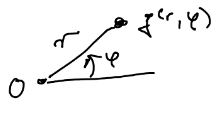
\includegraphics[width=0.2\linewidth]{figures/polarkoordinaten_abbildung}
            \label{fig:polarkoordinaten_abbildung}
        \end{figure}
        und \( f\maps \reals^2\to \reals \).
        \begin{align*}
            \totalderivative{f\circ g}(r,\phi)&=\totalderivative-{f}(g(r,\phi))\matrixmult \totalderivative-{g}(r,\phi
            )\\
            \totalderivative-{g}(r,\phi)&=\begin{pNiceMatrix} \partial_1 g(r,\phi) & \partial_2 g(r,\phi) \end{pNiceMatrix}=\begin{pNiceMatrix} \cos \phi & -r \sin \phi \\ \sin \phi & r\cos \phi \end{pNiceMatrix}.
        \end{align*}
        Somit 
        \begin{equation*}
            \begin{split}
                \totalderivative{f\circ g}(r,\phi)&=\begin{pNiceMatrix} \partial_1 f(g(r,\phi)) & \partial_2 f(g(r,\phi))  \end{pNiceMatrix}\matrixmult \begin{pNiceMatrix} \cos \phi & -r\sin \phi \\ \sin \phi & r\cos \phi \end{pNiceMatrix}\\
                &=\transpose{\begin{pNiceMatrix} \partial_1 f(g(r,\phi))\cdot \cos \phi+\partial_2(f(g(r,\phi)))\cdot\sin \phi \\
                -\partial_1 f(g(r,\phi))\cdot r\sin \phi+\partial_2 f(g(r,\phi))\cdot r \cos \phi \end{pNiceMatrix}}.
            \end{split}
        \end{equation*}
        Man schreibt dafür manchmal
        \begin{align*}
            \partial_r&=\cos \phi \partial_x+\sin \phi \partial_y\\
            \partial_\phi &=-r\sin \phi \partial_x+r\cos \phi\partial_y.
        \end{align*}
    \end{enumerate}
\end{beispiele}
Aber oft ist es \emph{viel} übersichtlicher, die partiellen Ableitungen \emph{nicht} nach den Namen der Variablen zu benennen, sondern durchzunummerieren!
\begin{beispiel*}
    \( f(x,y)=\frac{xy}{x^2+y^2} \) auf \( U=\reals^2\setminus \zeroset \).
    \begin{align*}
        \totalderivative-{f}(x,y)=\begin{pNiceMatrix} \frac{y(y^2)-x^2}{(x^2+y^2)}^2 \\ \frac{x(x^2-y^2)}{(x^2+y^2)} \end{pNiceMatrix}\\
        \totalderivative{f\circ g}(r,\phi)&\begin{aligned}[t]
            &=\frac{1}{r}(\cos^2 \phi-\sin^2 \phi)\begin{pNiceMatrix} \overbrace{-\sin \phi\cos \phi+\cos \phi \sin \phi}^{=0} \\ \underbrace{r\sin^2 \phi+r\cos^2\phi}_{=r} \end{pNiceMatrix}\\
            &=(0,\cos^2\phi -\sin^2\phi).
        \end{aligned}
    \end{align*}
    In diesem Fall rechnet man allerdings schneller direkt:
    \begin{align*}
        \totalderivative{f\circ g}(r,\phi)=\totalderivative{\tilde{f}}(r,\phi)=\cos \phi\cdot\sin \phi.
    \end{align*}
\end{beispiel*}
\begin{bemdef}
    Wir hatten allgemeiner gesehen:\\
    Ist \( f\maps U\to \reals^m \), \( U\subset \reals^n \) offen, differenzierbar in \( a \), so gilt
    \begin{align*}
        \partial_v f(a)\cdot \totalderivative-{f}(a)\matrixmult v\quad \forall v\in \reals^n.
    \end{align*}
    Ist speziell \( m=1 \), so definiert man
    \begin{align*}
        \grad-{f(a)}\definedas \transpose{\totalderivative-{f}(a)}=\begin{pNiceMatrix} \partial_1 f(a) \\ \Vdots \\ \partial_n f(a) \end{pNiceMatrix}\in \reals^n
    \end{align*}
    \enquote{Gradient von \( f \) in \( a \)}, und schreibt \( \partial_v f(a)=\scalarproduct{\grad-{f(a)}}{v} \).

    Ist \( \grad-{f(a)}\neq 0 \) und \( \norm{v}_{\text{E}}=1 \), so ist
    \begin{equation*}
        \scalarproduct{\grad-{f(a)}}{v}=\norm{\grad-{f(a)}}_{\text{E}}\cdot\cos \alpha,
    \end{equation*}
    wobei \( \alpha \) der zwischen \( \grad-{f(a)} \) und \( v \) in \( \reals^n \) eingeschlossene Winkel ist (in der durch die beiden Vektoren aufgespannten Ebene).

    Es folgt: \( \partial_v f(a) \) ist dann am größten, wenn \( v \) in die selbe Richtung zeigt wei \( \grad-{f(a)} \) \timplies der Gradient gibt die Richtung stärksten Anstiegs von \( f \) in \( a \) an.
\end{bemdef}
\begin{beispiel*}
    \( f(x)=x_1^2+x_2^2+2 \).
    \begin{figure}[H]
        \centering
        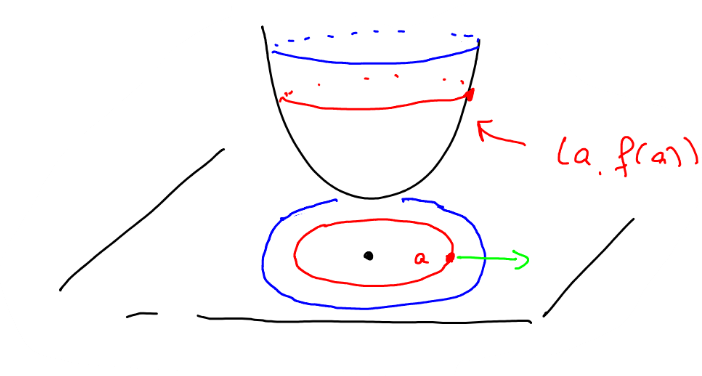
\includegraphics[width=0.5\linewidth]{figures/gradient_beispiel_parabel}
        \label{fig:gradient_beispiel_parabel}
    \end{figure}
\end{beispiel*}
\begin{beispiel*}
    \( f(x)=x^2 \).
    \begin{figure}[H]
        \centering
        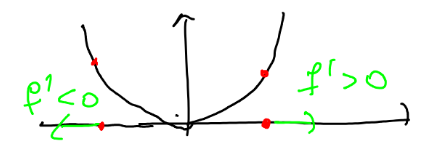
\includegraphics[width=0.4\linewidth]{figures/gradient_beispiel_parabel_2d}
        \caption*{}
        \label{fig:gradient_beispiel_parabel_2d}
    \end{figure}
    Ist \( f \) lediglich \emph{partiell differenzierbar}, \dh  die partiellen Ableitungen existieren auf \( U \), so definiert man dennoch
    \begin{equation*}
        \grad-{f(x)}=\transpose{(\partial_1 f(x),\dotsc, \partial_n f(x))}
    \end{equation*}
    als den Vektor der partiellen Ableitungen bei \( x \).
\end{beispiel*}
\begin{satz}\label{extremum_notwendige_bedingung}
    Sei \( f\maps U\to \reals \), \( U\subset \reals^n \) offen, \emph{partiell differenzierbar} auf \( U \). Sei \( a\in U \) ein \emph{lokales Maximum} (oder Minimum) von \( f \), \dh  \texists Umgebung \( V \) von \( a \) \sd \( f(x)\leq (a) \) (oder \( f(x)\geq f(a) \) für alle \( x\in V \)). Dann gilt
    \begin{equation*}
        \boxed{\grad-{f(a)}=0}.
    \end{equation*} 
\end{satz}
\begin{proof}
    Betrachte \( g_i(t)\definedas f(a+t e_i) \), \( i=1,\dotsc, n \), mit \( t\in \ointerval{-\varepsilon}{\varepsilon} \) \sd \( B_{\varepsilon}^{\norm{\cdot}}(a)\subset U \).
    \begin{figure}[H]
        \centering
        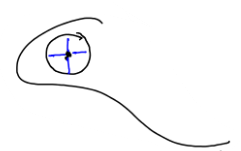
\includegraphics[width=0.5\linewidth]{figures/extrema_notwendige_bedingung_beweis_umgebung}
        \label{fig:extrema_notwendige_bedingung_beweis_umgebung}
    \end{figure}
    Ist \( a \) lokales Extremum (also lokales Maximum oder Minimum) von \( f\), so ist \( t=0 \) lokales Extremum von \( g_i \). Die \( g_i \) sind in \( t=0 \) differenzierbar, denn
    \begin{equation*}
        g_i'(0)=\partial_i f(a)\quad (\text{Definition Richtungsableitung})
    \end{equation*}
    \diff{1} \timplies \( g_i'(0)=0 \) \timplies \Beh.
\end{proof}
\begin{beispiele*}
    \begin{enumerate}
        \item \( f(x)=x_1^2+x_2^2+2 \). Außer in \( a=0 \) kann kein Extremum vorliegen.
        \item \( f(x,y)=\begin{cases}
            \frac{xy}{x^2+y^2}&(x,y)\neq (0,0)\\
            0 &(x,y)=(0,0).
        \end{cases} \). \( \partial_1 f(0)=0=\partial_2 f(0) \), also könnte \( 0 \) ein Extremum sein. Ist es aber nicht, da für \( x=y=\varepsilon>0 \) gilt \( f(\varepsilon,\varepsilon)=\frac{1}{2}>0 \) und für \( -x=y=\varepsilon>0 \). \( f(-\varepsilon,\varepsilon)=-\frac{1}{2}<0 \).
    \end{enumerate}
\end{beispiele*}
\begin{bemerkung*}
    Hinreichende Kriterien für das Vorliegen lokaler Extremstellen werden wir erst später kennen lernen. Wie in der \diff{1} benötigen wir dafür die 2.\ Ableitung.
\end{bemerkung*}
\begin{satz}\label{stetige_partielle_zu_ableitung}
     Sei \( f\maps U\to \reals \), \( U\subset \reals^n \) offen. Existieren alle partiellen Ableitungen \( \partial_j f(x) \) für alle \( x\in U \), \emph{und} sind sie stetig in \( a\in U \), so ist \( f \) in \( a \) differenzierbar.
\end{satz}
\begin{proof}
    Wir wählen ein Norm \( \norm{\cdot} \) auf \( \reals^n \). \( U \) offen \timplies \texists \( \delta>0 \) \sd  \( B_{\delta}^{\norm{\cdot}}(a)\subset U \). Sei \( h\in B_{\delta}^{\norm{\cdot}}(0) \), also \( a+h\in B_{\delta}^{\norm{\cdot}}(a) \). Setze
    \begin{equation*}
        x^{(j)}\definedas a+\sum_{i=1}^{j} h_i e_i \in \reals^n\quad j=0,\dotsc,n,
    \end{equation*}
    also \( x^{(0)}=a \), \( x^{(1)}=(a_1+h_1,a_2,\dotsc, a_n),\dotsc, x^{(n)}=a+h \). Es ist \( x^{(j)}-x^{(j-1)}=(0,\dotsc,0,h_j,0,\dotsc,0) \) \timplies (MWS, \diff{1}) \texists \( \eta_j\in \interval{0}{1} \) \sd 
    \begin{align*}
        &f(x)=\partial_j f(\underbrace{x_1^{(j-1)},\dotsc,x_{j-1}^{(j-1)},x_j^{(j-1)}+\eta_j h_j,a_{j+1}, \dotsc, a_n}_{x^{j-1}+\eta_j h_j e_j\defines y^{(j)}})\cdot h_j\\
        \implies &f(a+h)-f(a)\begin{aligned}[t]
            &=\sum_{j=1}^{n}(f(x^{(j)})-f(x^{(j-1)}))\\
            &=\sum_{j=1}^{n}\partial_j f(y^{(j)}) h_j\\
            &\needed{=} \begin{pNiceMatrix} \partial_1 f(a) & \Cdots & \partial_n f(a) \end{pNiceMatrix}\begin{pNiceMatrix} h_1 \\ \Vdots \\ h_n \end{pNiceMatrix}+ \underline{R}_a(h)
        \end{aligned}
    \end{align*}
    also ist
    \begin{align*}
        &\underline{R}_a(h)=\sum_{j=1}^{n} (\partial_j f(y^{(j)})-A_j)h_j\quad A=\partial_j f(a)\\
        \overset{\text{CS}}{\implies}&\frac{\abs{\underline{R}_a(h)}}{\norm{h}}\leq C\norm{(\partial_1 f(y^{(1)})-A_1,\dotsc,\partial_n f(y^{(n)})-A_n)}_{\text{E}}\goesto 0 \quad h\goesto 0,
    \end{align*}
    denn \( \lim_{h\goesto 0}y^{(j)}=\lim_{h\goesto 0}x^{(j-1)}+\eta_j h_j e_j=a \) (in \( \reals^n \)) und die \( \partial_j f \) sind in \( a \) stetig nach Voraussetzung, \sd
    \begin{align*}
        \lim_{h \goesto 0}\partial_j f(y^{(j)})=(\partial_j f)(\lim y^{(j)})=\partial_j f(a).
    \end{align*}
\end{proof}
\begin{bemerkungen}
    \begin{enumerate}
        \item \label{stetig_differenzierbar} Man sieht: Sind die \( \partial_j  \) auf \( U \) stetig, so ist auch die Ableitung \( x\mapsto \totalderivative-{f}(x) \) eine stetige Abbildung \( U\to \Mat(m\times n, \reals) \). Man sagt in dem Fall: \( f \) ist \emph{stetig differenzierbar}.
        \item \label{stetige_partielle_zu_ableitung:nicht_nur_reell} Die Einschränkung auf reellwertige Funktionen ist keine, denn: \( f\maps U\to \reals^m \) ist genau dann in \( a\in U\subset \reals^n \) differenzierbar, wenn alle Komponentenfunktionen \( f_j\maps U\to \reals \) differenzierbar sind (\( j=1,\dotsc, m \))-
    \end{enumerate}
\end{bemerkungen}
\begin{proof}
    \begin{proofdescription}
        \item[\ref{stetige_partielle_zu_ableitung:nicht_nur_reell}] \( f(a+h)=f(a)+A\matrixmult h+\underline{R}(h) \), \( A_{ji}=\partial_j f_j(a) \) 
        \begin{equation*}
            \iff f_j(a+h)=f_(a)+\begin{pNiceMatrix} \partial_1 f_j(a) & \Cdots & \partial_n f_j(a) \end{pNiceMatrix}\matrixmult h+\underline{R}_j(h)\quad \forall j=1,\dotsc, m
        \end{equation*}
        und
        \begin{equation*}
            \frac{\underline{R}(h)}{\norm{h}}\goesto 0 \text{ in }\reals^m\iff \frac{\explicitnorm{\max}{\underline{R}(h)}}{\norm{h}}\goesto 0\iff \frac{\abs{R}_j(h)}{\norm{h}}\goesto 0\quad j=1,\dotsc,m.
        \end{equation*}
        \item[\ref{stetig_differenzierbar}] Dito: \( U\to \Mat(m\times n,\reals) \) ist stetig \tiff alle Komponentenfunktionen \( A_{ij}\maps U\to \reals \) sind stetig.
    \end{proofdescription}
    
\end{proof}
\begin{bemerkung*}
    Stetig differenzierbar \timplies differenzierbar \timplies partiell differenzierbar.

    Die Umkehrungen sind im Allgemeinen falsch.
\end{bemerkung*}
\begin{bemerkung*}[Erinnerung (\diff{1}) MWS]
    \( f\maps I\to \reals \) differenzierbar, \( I \) Intervall, \texists \( \epsilon\in \interval{0}{1} \) \sd
    \begin{equation*}
        f(a+h)-f(a)=f'(a+\eta h)\cdot h.
    \end{equation*}
    Ist \( f \) stetig differenzierbar, folgt aus dem Hauptsatz der Differenzial- und Integralrechnung eine andere Variante:
    \begin{equation*}
        f(a+h)-f(a)=\Integrate{f'(u)}{u,a,a+h}=\Integrate{f'(a+th)}{t,0,1}\cdot h.
    \end{equation*}
\end{bemerkung*}
Eine analoge Aussage wollen wir nun im \( \reals^n \) beweisen.
\begin{definition*}
    Sei \( A\maps I\to \reals^k \),\( I\subset \reals \) Intervall, stetig. Dann ist das \emph{Integral von \( A \)} über \( \interval{a}{b}\in I \) definiert als
    \begin{equation*}
        \Integrate{A(t)}{t,a,b}=\begin{pNiceMatrix} \Integrate{A_1(t)}{t,a,b} \\ \Vdots \\ \Integrate{A_k(t)}{t,a,b} \end{pNiceMatrix}.
    \end{equation*}
    Insbesondere ist das Integral einer matrixwertigen, stetigen Funktion \( A\maps I\to \Mat(m\times n,\reals) \) die Matrix, deren Einträge gleich den Integralen der Komponenten von \( A(t) \) ist, also
    \begin{equation*}
        \Integrate{A(t)}{t,a,b}=\left( \Integrate{A_{ij}(t)}{t,a,b} \right)_{\substack{1\leq i\leq m\\1\leq j\leq n}}.
    \end{equation*}
\end{definition*}
\begin{satz}\label{verbindungsstrecke_integral_mws}
    Sei \( f\maps U\to \reals^m \), \( U\subset \reals^n \), stetig differenzierbar. Sei \( a\in U \) und \( h\in \reals^n \) \sd  die Verbindungsstrecke
    \begin{equation*}
        \Set{a+th|t\in \interval{0}{1}}\subset U.
    \end{equation*}
    Dann gilt:
    \begin{equation*}
        f(a+h)-f(a)=\left( \Integrate{\totalderivative-{f}(a+th)}{t,0,1} \right)\matrixmult h.
    \end{equation*}
    \begin{figure}[H]
        \centering
        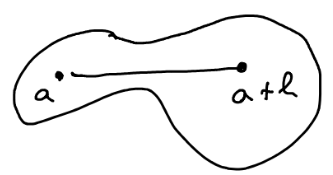
\includegraphics[width=0.5\linewidth]{figures/mws_integral_verbindungsstrecke}
        \label{fig:mws_integral_verbindungsstrecke}
    \end{figure}
\end{satz}
\begin{proof}
    Wir arbeiten zeilenweise, betrachten also die Komponentenfunktionen. Setze \( g_i(t)\definedas f_i(a+th) \). Dann ist \( g_i \) stetig differenzierbar, denn mit der Kettenregel gilt \( g_i'(t)=\totalderivative-{f}_i(a+th)\matrixmult h \).
    \begin{equation*}
        \begin{split}
            f_i(a+h)-f_i(a)&=g_i(1)-g_i(0)\\
            &=\Integrate{g_i'(t)}{t,0,1}\\
            &=\Integrate{\totalderivative-{f}_i(a+th)\matrixmult h}{t,0,1}\\
            &\explain[big]{\int \text{ linear}}{=}\underbrace{\left( \Integrate{\totalderivative-{f}_i(a+th)}{t,0,1} \right)}_{(1\times n)\text{-Matrix}}\matrixmult h\quad 1\leq i \leq m.
        \end{split}
    \end{equation*}
    Dies sind die Zeilen der Matrix \( \Integrate{\totalderivative-{f}(a+th)}{t,0,1} \).
\end{proof}
\begin{folgerung}\label{differenz_abschaetzung_ableitung_verbindungsstrecke}
    Unter den Voraussetzungen von \ref{verbindungsstrecke_integral_mws} gilt \( \norm{f(x+h)-f(x)}_{\text{E}}\leq C\norm{h} \) mit
    \begin{equation*}
        C=\sup_{t\in \interval{0}{1}}\norm{\totalderivative-{f}(x+th)}_{\text{op}}.
    \end{equation*}
\end{folgerung}
Der Beweis benötigt noch ein Lemma:
\begin{lemma}\label{integral_norm_dreiecksungleichung}
    Sei \( v\maps \interval{a}{b}\to \reals^m \) stetig. Dann gilt
    \begin{equation*}
        \norm{\Integrate{v(t)}{t,a,b}}_{\text{E}}\leq \Integrate{\norm{v(t)}_{\text{E}}}{t,a,b}.
    \end{equation*}
\end{lemma}
\begin{proof}
    Sei \( \reals^m\ni u=\Integrate{v(t)}{t,a,b} \). Dann gilt
    \begin{equation*}
        \begin{split}
            \norm{n}_{\text{E}}^2&=\scalarproduct{u}{u}\\
            &=\scalarproduct{\Integrate{v(t)}{t,a,b}}{u}\\
            &\explain[big]{\text{Linearität}}{=}\Integrate{\scalarproduct{v(t)}{u}}{t,a,b}\\
            &\explain{\text{Monotonie und C-S}}{\leq}\Integrate{\norm{v(t)}_{\text{E}}\norm{u}_{\text{E}}}{t,a,b}\\
            &=\norm{u}_{\text{E}} \Integrate{\norm{v(t)}_{\text{E}}}{t,a,b}.
        \end{split}
    \end{equation*}
\end{proof}
\begin{bemerkungen*}
    \begin{enumerate}
        \item Wegen der Äquivalenz aller Normen auf \( \reals^n \) gilt diese Abschätzung ebenso wie \thref{differenz_abschaetzung_ableitung_verbindungsstrecke} auch für beliebige Normen auf \( \reals^n \):
        \begin{equation*}
            \begin{split}
                \norm{\Integrate{v(t)}{t}}&\leq C_1\norm{\Integrate{v(t)}{t}}_{\text{E}}\\
                &\leq C_1\Integrate{\norm{v(t)}_{\text{E}}}{t}\\
                &\leq C_1 C_2 \Integrate{\norm{v(t)}}{t}.
            \end{split}
        \end{equation*}
        \item Es folgt, dass für
        \begin{equation*}
            X=(\explain{\sup\norm{v(t)}<\infty \text{, da \( \interval{a}{b} \) kompakt und \( v \) stetig.}}{\stetigefunktionen}(\interval{a}{b},\reals^k),\supnorm{\cdot}),
        \end{equation*}
        \( \int_a^b\maps X\to \reals^k \) stetig ist, denn \( \int_a^b \) ist linear und
        \begin{equation*}
            \begin{split}
                \norm{\int_a^b}_{\text{op}}&=\sup_{0\neq v \in \stetigefunktionen}\quot{\norm{\Integrate{v(t)}{t,a,b}}}{\supnorm{v}}\\
                &\leq C\sup_{v\neq 0}\quot{\norm{\Integrate{v(t)}{t,a,b}}_{\text{E}}}{\supnorm{v}}\\
                &\leq C\sup_{v\neq 0}\quot{\Integrate{\norm{v(t)}_{\text{E}}}{t,a,b}}{\supnorm{v}}\\
                &\leq \tilde{C}(b-a),
            \end{split}
        \end{equation*}
        denn \( \norm{v(t)}_{\text{E}}\leq \sup_{t}\norm{v(t)}_\text{E}\leq C_0\sup_t\norm{v(t)}=C_0\supnorm{v} \).
    \end{enumerate}
\end{bemerkungen*}
\begin{proof}[Beweis von \thref{differenz_abschaetzung_ableitung_verbindungsstrecke}]
    \begin{equation*}
        \begin{split}
            \norm{f(x+h)-f(x)}_{\text{E}}&\leq \Integrate{\norm{\totalderivative-{f}(x+th)\matrixmult h}_{\text{E}}}{t,0,1}\\
            &\leq \Integrate{\norm{\totalderivative-{f}(x+th)}_{\text{op}}\matrixmult \norm{h}_{\text{E}}}{t,0,1}.
        \end{split}
    \end{equation*}
    Das Supremum wird angenommen, da \( t\mapsto \norm{\totalderivative-{f}(x+th)}_{\text{op}} \) stetig ist und \( \interval{0}{1} \) kompakt.
\end{proof}
\section*{Implizite Funktionen} Eine Anwendung der Kettenregel

Manchmal ist es einfacher, eine \( 1 \)-dimensionale Ableitung über eine Ableitung einer höherdimensionalen Funktion zu berechnen. Betrachte etwa zwei differenzierbare Funktionen \( f\maps U\to \reals \), \( U\subset \reals^2 \) offen, und \( g\maps I\to \reals \). Sei \( \Gamma_g\subset U \) und es gelte
\begin{equation*}
    f(\underbrace{t,g(t)}_{\in \Gamma_g})=0\quad \forall t\in I.
\end{equation*}
Dann gilt (Kettenregel!) (mit \( \Id(t)=t \)):
\begin{equation*}
    \begin{split}
        0&=D*{f\circ \begin{pNiceMatrix} \Id \\ g \end{pNiceMatrix}}(t)\\
         &=\totalderivative-{f}\left( (t,g(t)) \right)\matrixmult \totalderivative-{\begin{pNiceMatrix} \Id \\ g \end{pNiceMatrix}}(t)\\
         &=\begin{pNiceMatrix} \partial_1 f(t,g(t)) & \partial_2 f(t,g(t)) \end{pNiceMatrix}\matrixmult \begin{pNiceMatrix} 1 \\ g'(t) \end{pNiceMatrix}
    \end{split}
\end{equation*}
\timplies Ist \(  \partial_2 f(t,g(t))\neq 0 \), so gilt
\begin{align*}
    g'(t)=-\frac{\partial_1 f(t,g(t))}{\partial_2 g(t,g(t))}.
\end{align*}
\begin{beispiel*}
    \( g\maps \ointerval{0}{1}\to \reals \), \( g(t)=\arcsin \sqrt{1-t^3} \), also \( \sin(g(t))=\sqrt{1-t^3} \), also \( (\sin(g(t)))^2=1-t^3 \). Also gilt \( f(t,g(t))=0 \) für
    \begin{align*}
        f(x,y)&=(\sin y)^2-1+x^3\\
        \totalderivative-{f}(x,y)&=(3x^2,2\sin y \cos y)\\
        \implies g'(t)&\begin{aligned}[t]
            &=-\frac{3t^2}{2\sin(g(t))\underbrace{\cos(g(t))}_{>0,}}
            \intertext{da \( t\in \ointerval{0}{1} \) und \( \sqrt{1-t^3}\in \ointerval{0}{1} \), somit \( g(t)\in \ointerval{0}{\quot{\pi}{2}} \) \timplies \( \cos g(t)=+\sqrt{1-\underbrace{\sin^2 g(t)}_{1-t^3}}=\sqrt{t^3} \)}
            &=-\frac{3t^2}{2\sqrt{1-t^3}\sqrt{t^3}}.
        \end{aligned}
    \end{align*}
\end{beispiel*}